\documentclass[11pt,compress,t,notes=noshow, xcolor=table]{beamer}
\usepackage[]{graphicx}\usepackage[]{color}
% maxwidth is the original width if it is less than linewidth
% otherwise use linewidth (to make sure the graphics do not exceed the margin)
\makeatletter
\def\maxwidth{ %
  \ifdim\Gin@nat@width>\linewidth
    \linewidth
  \else
    \Gin@nat@width
  \fi
}
\makeatother

\definecolor{fgcolor}{rgb}{0.345, 0.345, 0.345}
\newcommand{\hlnum}[1]{\textcolor[rgb]{0.686,0.059,0.569}{#1}}%
\newcommand{\hlstr}[1]{\textcolor[rgb]{0.192,0.494,0.8}{#1}}%
\newcommand{\hlcom}[1]{\textcolor[rgb]{0.678,0.584,0.686}{\textit{#1}}}%
\newcommand{\hlopt}[1]{\textcolor[rgb]{0,0,0}{#1}}%
\newcommand{\hlstd}[1]{\textcolor[rgb]{0.345,0.345,0.345}{#1}}%
\newcommand{\hlkwa}[1]{\textcolor[rgb]{0.161,0.373,0.58}{\textbf{#1}}}%
\newcommand{\hlkwb}[1]{\textcolor[rgb]{0.69,0.353,0.396}{#1}}%
\newcommand{\hlkwc}[1]{\textcolor[rgb]{0.333,0.667,0.333}{#1}}%
\newcommand{\hlkwd}[1]{\textcolor[rgb]{0.737,0.353,0.396}{\textbf{#1}}}%
\let\hlipl\hlkwb

\usepackage{framed}
\makeatletter
\newenvironment{kframe}{%
 \def\at@end@of@kframe{}%
 \ifinner\ifhmode%
  \def\at@end@of@kframe{\end{minipage}}%
  \begin{minipage}{\columnwidth}%
 \fi\fi%
 \def\FrameCommand##1{\hskip\@totalleftmargin \hskip-\fboxsep
 \colorbox{shadecolor}{##1}\hskip-\fboxsep
     % There is no \\@totalrightmargin, so:
     \hskip-\linewidth \hskip-\@totalleftmargin \hskip\columnwidth}%
 \MakeFramed {\advance\hsize-\width
   \@totalleftmargin\z@ \linewidth\hsize
   \@setminipage}}%
 {\par\unskip\endMakeFramed%
 \at@end@of@kframe}
\makeatother

\definecolor{shadecolor}{rgb}{.97, .97, .97}
\definecolor{messagecolor}{rgb}{0, 0, 0}
\definecolor{warningcolor}{rgb}{1, 0, 1}
\definecolor{errorcolor}{rgb}{1, 0, 0}
\newenvironment{knitrout}{}{} % an empty environment to be redefined in TeX

\usepackage{alltt}
\newcommand{\SweaveOpts}[1]{}  % do not interfere with LaTeX
\newcommand{\SweaveInput}[1]{} % because they are not real TeX commands
\newcommand{\Sexpr}[1]{}       % will only be parsed by R
\newcommand{\xmark}{\ding{55}}%


\usepackage[english]{babel}
\usepackage[utf8]{inputenc}

\usepackage{dsfont}
\usepackage{verbatim}
\usepackage{amsmath}
\usepackage{amsfonts}
\usepackage{amssymb}
\usepackage{bm}
\usepackage{csquotes}
\usepackage{multirow}
\usepackage{longtable}
\usepackage{booktabs}
\usepackage{enumerate}
\usepackage[absolute,overlay]{textpos}
\usepackage{psfrag}
\usepackage{algorithm}
\usepackage{algpseudocode}
\usepackage{eqnarray}
\usepackage{arydshln}
\usepackage{tabularx}
\usepackage{placeins}
\usepackage{tikz}
\usepackage{setspace}
\usepackage{colortbl}
\usepackage{mathtools}
\usepackage{wrapfig}
\usepackage{bm}
\usepackage{amsmath}
\usepackage{pifont}
\usepackage{xcolor} %colored math symbols

\usetikzlibrary{shapes,arrows,automata,positioning,calc,chains,trees, shadows}
\tikzset{
  %Define standard arrow tip
  >=stealth',
  %Define style for boxes
  punkt/.style={
    rectangle,
    rounded corners,
    draw=black, very thick,
    text width=6.5em,
    minimum height=2em,
    text centered},
  % Define arrow style
  pil/.style={
    ->,
    thick,
    shorten <=2pt,
    shorten >=2pt,}
}

\usepackage{subfig}

% Defines macros and environments
\usepackage{../../style/lmu-lecture}


\let\code=\texttt
\let\proglang=\textsf

\setkeys{Gin}{width=0.9\textwidth}

\setbeamertemplate{frametitle}{\expandafter\uppercase\expandafter\insertframetitle}

\usepackage{bbm}
% basic latex stuff
\newcommand{\pkg}[1]{{\fontseries{b}\selectfont #1}} %fontstyle for R packages
\newcommand{\lz}{\vspace{0.5cm}} %vertical space
\newcommand{\dlz}{\vspace{1cm}} %double vertical space
\newcommand{\oneliner}[1] % Oneliner for important statements
{\begin{block}{}\begin{center}\begin{Large}#1\end{Large}\end{center}\end{block}}


%new environments
\newenvironment{vbframe}  %frame with breaks and verbatim
{
 \begin{frame}[containsverbatim,allowframebreaks]
}
{
\end{frame}
}

\newenvironment{vframe}  %frame with verbatim without breaks (to avoid numbering one slided frames)
{
 \begin{frame}[containsverbatim]
}
{
\end{frame}
}

\newenvironment{blocki}[1]   % itemize block
{
 \begin{block}{#1}\begin{itemize}
}
{
\end{itemize}\end{block}
}

\newenvironment{fragileframe}[2]{  %fragile frame with framebreaks
\begin{frame}[allowframebreaks, fragile, environment = fragileframe]
\frametitle{#1}
#2}
{\end{frame}}


\newcommand{\myframe}[2]{  %short for frame with framebreaks
\begin{frame}[allowframebreaks]
\frametitle{#1}
#2
\end{frame}}

\newcommand{\remark}[1]{
  \textbf{Remark:} #1
}


\newenvironment{deleteframe}
{
\begingroup
\usebackgroundtemplate{
\includegraphics[width=\paperwidth,height=\paperheight]{../style/color/red.png}}
 \begin{frame}
}
{
\end{frame}
\endgroup
}
\newenvironment{simplifyframe}
{
\begingroup
\usebackgroundtemplate{
\includegraphics[width=\paperwidth,height=\paperheight]{../style/color/yellow.png}}
 \begin{frame}
}
{
\end{frame}
\endgroup
}\newenvironment{draftframe}
{
\begingroup
\usebackgroundtemplate{
\includegraphics[width=\paperwidth,height=\paperheight]{../style/color/green.jpg}}
 \begin{frame}
}
{
\end{frame}
\endgroup
}
% https://tex.stackexchange.com/a/261480: textcolor that works in mathmode
\makeatletter
\renewcommand*{\@textcolor}[3]{%
  \protect\leavevmode
  \begingroup
    \color#1{#2}#3%
  \endgroup
}
\makeatother


\input{../../latex-math/basic-math}
\input{../../latex-math/basic-ml}
\input{../../latex-math/ml-nn}

\title{Deep Learning}

\date{}

\begin{document}
\newcommand{\titlefigure}{plots/GAN01.png}
%modify picture
\newcommand{\learninggoals}{
  \item architecture of a GAN
  \item minimax loss
  \item training a GAN
  %\item adversarial training 
  %\item projected gradient descent
  %\item fast gradient sign method
  %\item Principal component analysis
}


\lecturechapter{Introduction to Generative Adversarial Networks (GANs)}
\lecture{I2DL}


%\begin{frame} {Generative Adversarial Networks (GANs)}
%
%Generative adversarial networks
%\begin{itemize}
%\item define the generative model as in VAEs,
%\item but approach problem of learning a directed generative model $p(\mathbf{x}| \mathbf{z})$ from a totally different perspective.
%\vspace{1mm}
%\end{itemize}
%\begin{figure}
%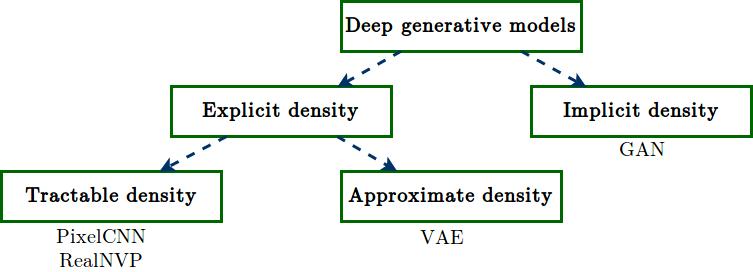
\includegraphics[width=8cm]{plots/taxonomy.png}
%\tiny{\\Taxonomy of Generative Model}
%\end{figure}

%\end{frame}

\begin{frame} {What is a GAN?}
    \begin{figure}
    \centering
    \scalebox{0.52}{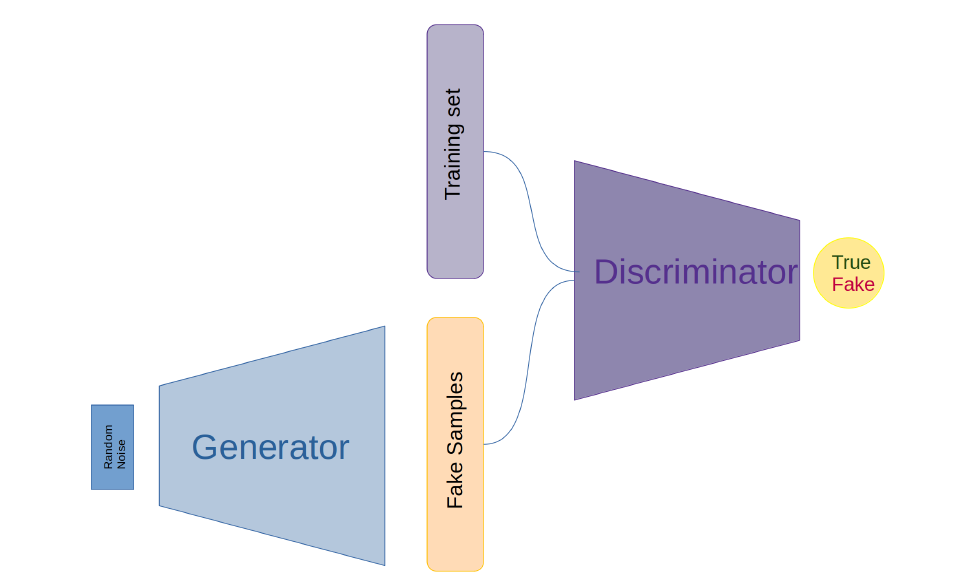
\includegraphics{plots/GAN01.png}}
    \end{figure}
    \begin{itemize}
    \item A  \emph{generative adversarial network} (GAN)  consists of two DNNs:
    \begin{itemize}
    \item generator 
    \item discriminator
    \end{itemize}
    \item Generator transforms random noise vector into fake sample. %in a given domain.
    \item Discriminator gets real and fake samples  as input and outputs %a number between 0 and 1 indicating the 
    probability of the input being real.
    \end{itemize}
    \end{frame}
    
    \begin{frame} {What Is a GAN?}
\begin{figure}
\centering
\scalebox{0.4}{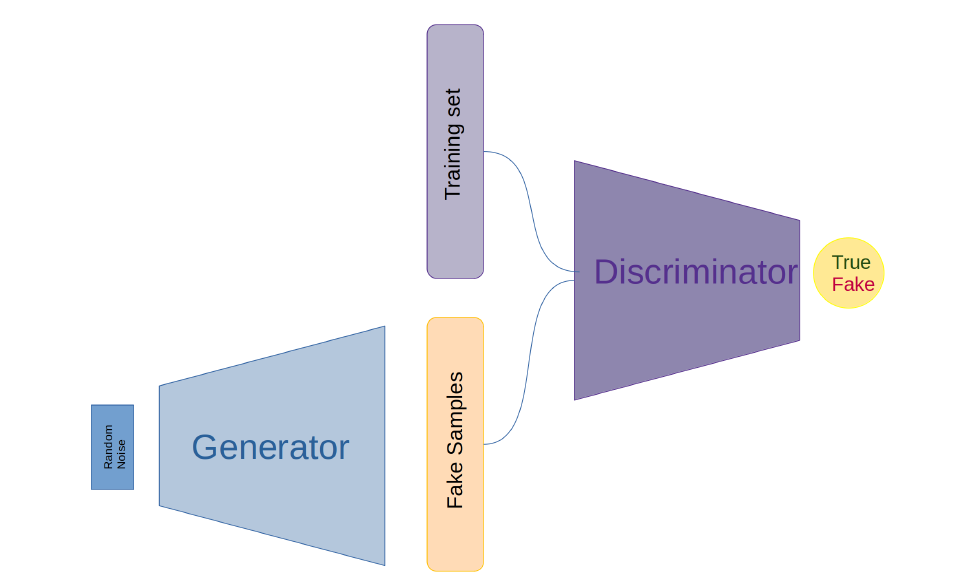
\includegraphics{plots/GAN01.png}}
\end{figure}
\begin{itemize}
\item Goal of generator: fool discriminator into thinking that the synthesized samples are real.
\item Goal of discriminator: recognize real samples and not being fooled by  generator.
\item This sets off an arms race. As the generator gets better at producing realistic samples, the discriminator is forced to get better at detecting the fake samples which in turn forces the generator to get even better at producing realistic samples and so on.
\end{itemize}
\end{frame}

\begin{frame} {Fake currency illustration}
\vspace{1mm}
The generative model can be thought of as analogous to a team of counterfeiters, trying to produce fake currency and use it without detection, while the discriminative model is analogous to the police, trying to detect the counterfeit currency. Competition in this game drives both teams to improve their methods until the counterfeits are indistinguishable from the genuine articles. \\
\hspace{45mm} -Ian Goodfellow

\begin{figure}
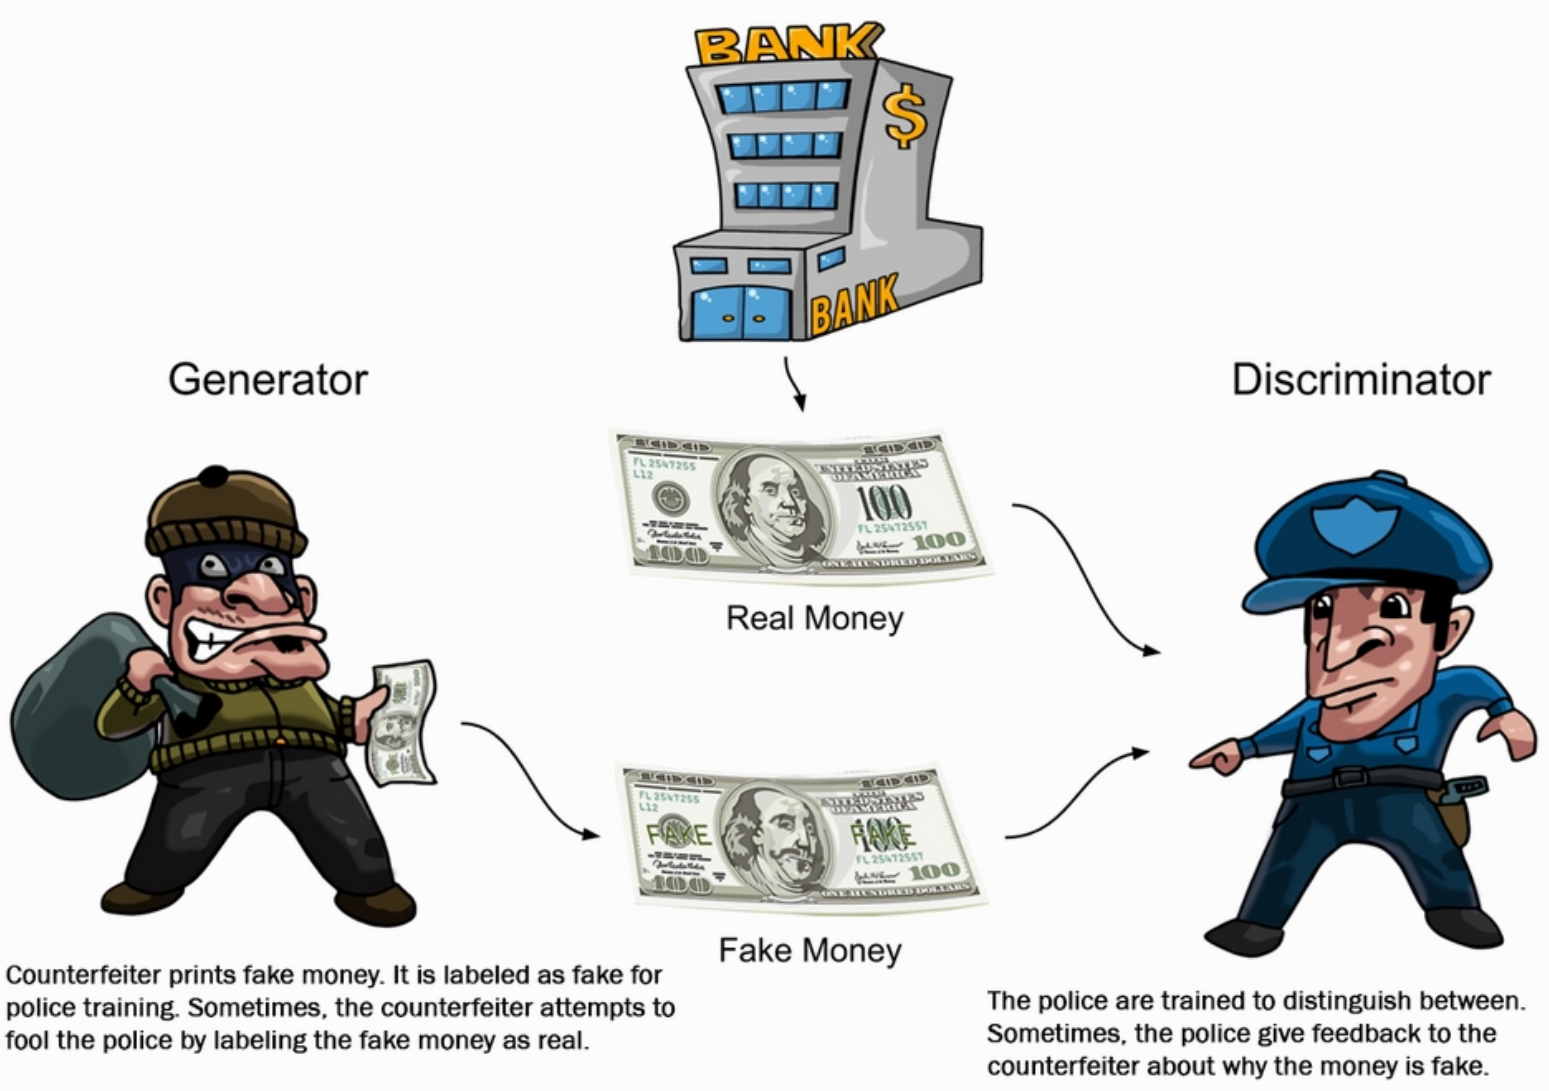
\includegraphics[width=5cm]{plots/counterfeiters.png}
\tiny{\\Image created by Mayank Vadsola}
\end{figure}

\end{frame}



\section{GAN Training}

\begin{frame} {Minimax Loss for GANs}
  \begin{tcolorbox}
  $\min \limits_G \max  %\limits_D V(D,G)
  = \E_{\mathbf{x}\sim p_{\text{data}(\mathbf{x})}}[\log D(\mathbf{x})] + \E_{\mathbf{z}\sim p(\mathbf{z})}[\log (1 - D(G(\mathbf{z})))]$
  \end{tcolorbox}
   \begin{itemize}
  \vspace{6mm}
      \item $p_{\text{data}(\mathbf{x})}$ is our target, the data distribution.
  \vspace{6mm}
  \item The generator is a neural network mapping a latend random vector $\mathbf{z}$ to generated sample $G(\mathbf{z})$. Even if the generator is a determinisic function, we have random outputs, i.e.~variability. 
      %\item Because a neural network (the generator) is a deterministic function, we feed a latent random vector $\mathbf{z}$ to the generator to induce variability in its outputs.
  \vspace{6mm}
      \item $p(\mathbf{z})$ is usually a uniform distribution or an isotropic Gaussian. It is typically fixed and not adapted during training.

   \end{itemize}
\end{frame}

\begin{frame} {Minimax Loss for GANs}
  \begin{tcolorbox}
    $\min \limits_G \max %\limits_D V(D,G) = 
    \E_{\mathbf{x}\sim p_{\text{data}(\mathbf{x})}}[\log D(\mathbf{x})] + \E_{\mathbf{z}\sim p(\mathbf{z})}[\log (1 - D(G(\mathbf{z})))]$
  \end{tcolorbox}
  \begin{itemize}
  \vspace{6mm}
    \item $G(\mathbf{z})$ is the output of the generator for a given state $\mathbf{z}$ of the latent variables.
  \vspace{6mm}
      \item $D(\mathbf{x})$ is the output of the discriminator for a real sample $\mathbf{x}$.
  \vspace{6mm}
      \item $D(G(\mathbf{z}))$ is the output of the discriminator for a fake sample $G(\mathbf{z})$ synthesized by the generator.
  \end{itemize}
\end{frame}


\begin{frame} {Minimax Loss for GANs}
  \begin{tcolorbox}
    $\min \limits_G \max  %\limits_D V(D,G) 
    = \E_{\mathbf{x}\sim p_{\text{data}(\mathbf{x})}}[\log D(\mathbf{x})] + \E_{\mathbf{z}\sim p(\mathbf{z})}[\log (1 - D(G(\mathbf{z})))]$
  \end{tcolorbox}
  \begin{itemize}
    \item $\E_{\mathbf{x}\sim p_{\text{data}(\mathbf{x})}}[\log D(\mathbf{x})]$ is the log-probability of correctly classifying real data points as real. 
  \vspace{2mm}
    \item $\E_{\mathbf{z}\sim p(\mathbf{z})}[\log (1 - D(G(\mathbf{z})))]$ is the log-probability of correctly classifying fake samples as fake.
  \vspace{2mm}
    \item With each gradient update, the discriminator tries to push $D(\mathbf{x})$ toward 1 and $D(G(\mathbf{z})))$ toward 0. This is the same as maximizing V(D,G).
  \vspace{2mm}
    \item The generator  only has control over $D(G(\mathbf{z}))$ and tries to push that toward 1 with each gradient update. This is the same as minimizing V(D,G).
  \end{itemize}
\end{frame}

\begin{frame} {GAN training : Pseudocode}
  \begin{algorithm}[H]
  \footnotesize
    \caption{Minibatch stochastic gradient descent training of GANs. Amount of training iterations, amount of discriminator updates $k$ }
    \begin{algorithmic}[1]
      \For{number of training iterations}
        \For{k steps}
          \State Sample minibatch of $m$ samples $\{\mathbf{z}^{(1)} \ldots \mathbf{z}^{(m)}$\} from  prior $p_g(\mathbf{z})$
          \State Sample minibatch of $m$ examples $\{\mathbf{x}^{(1)} \ldots \mathbf{x}^{(m)}$\} from  training data 
 %generating distribution $p_{\text{data}}(\mathbf{x})$.
          \State Update discriminator by ascending the stochastic gradient: \item[]
  \hspace{2.5 cm}          $\nabla_{{\theta}_d} \frac {1}{m} \sum \limits_{i=1} \limits^{m} \left [ \log D(\mathbf{x}^{(i)}) + \log (1 - D(G(\mathbf{z}^{(i)}))) \right]$
            % + \log (1 - D(G(\mathbf{z}^{(i)})))}\right]$
        \EndFor
        \State Sample minibatch of $m$ noise samples $\{\mathbf{z}^{(1)} \ldots \mathbf{z}^{(m)}$\} from the noise prior $p_g(\mathbf{z})$
        \State Update generator by descending the stochastic gradient: \item[]
   \hspace{2.5 cm}       $\nabla_{{\theta}_g} \frac {1}{m} \sum \limits_{i=1} \limits^{m} \log (1 - D(G(\mathbf{z}^{(i)})))$
      \EndFor
    \end{algorithmic}
  \end{algorithm}
\end{frame}


\begin{frame} {GAN training: Illustration}
\begin{figure}
\centering
\scalebox{0.75}{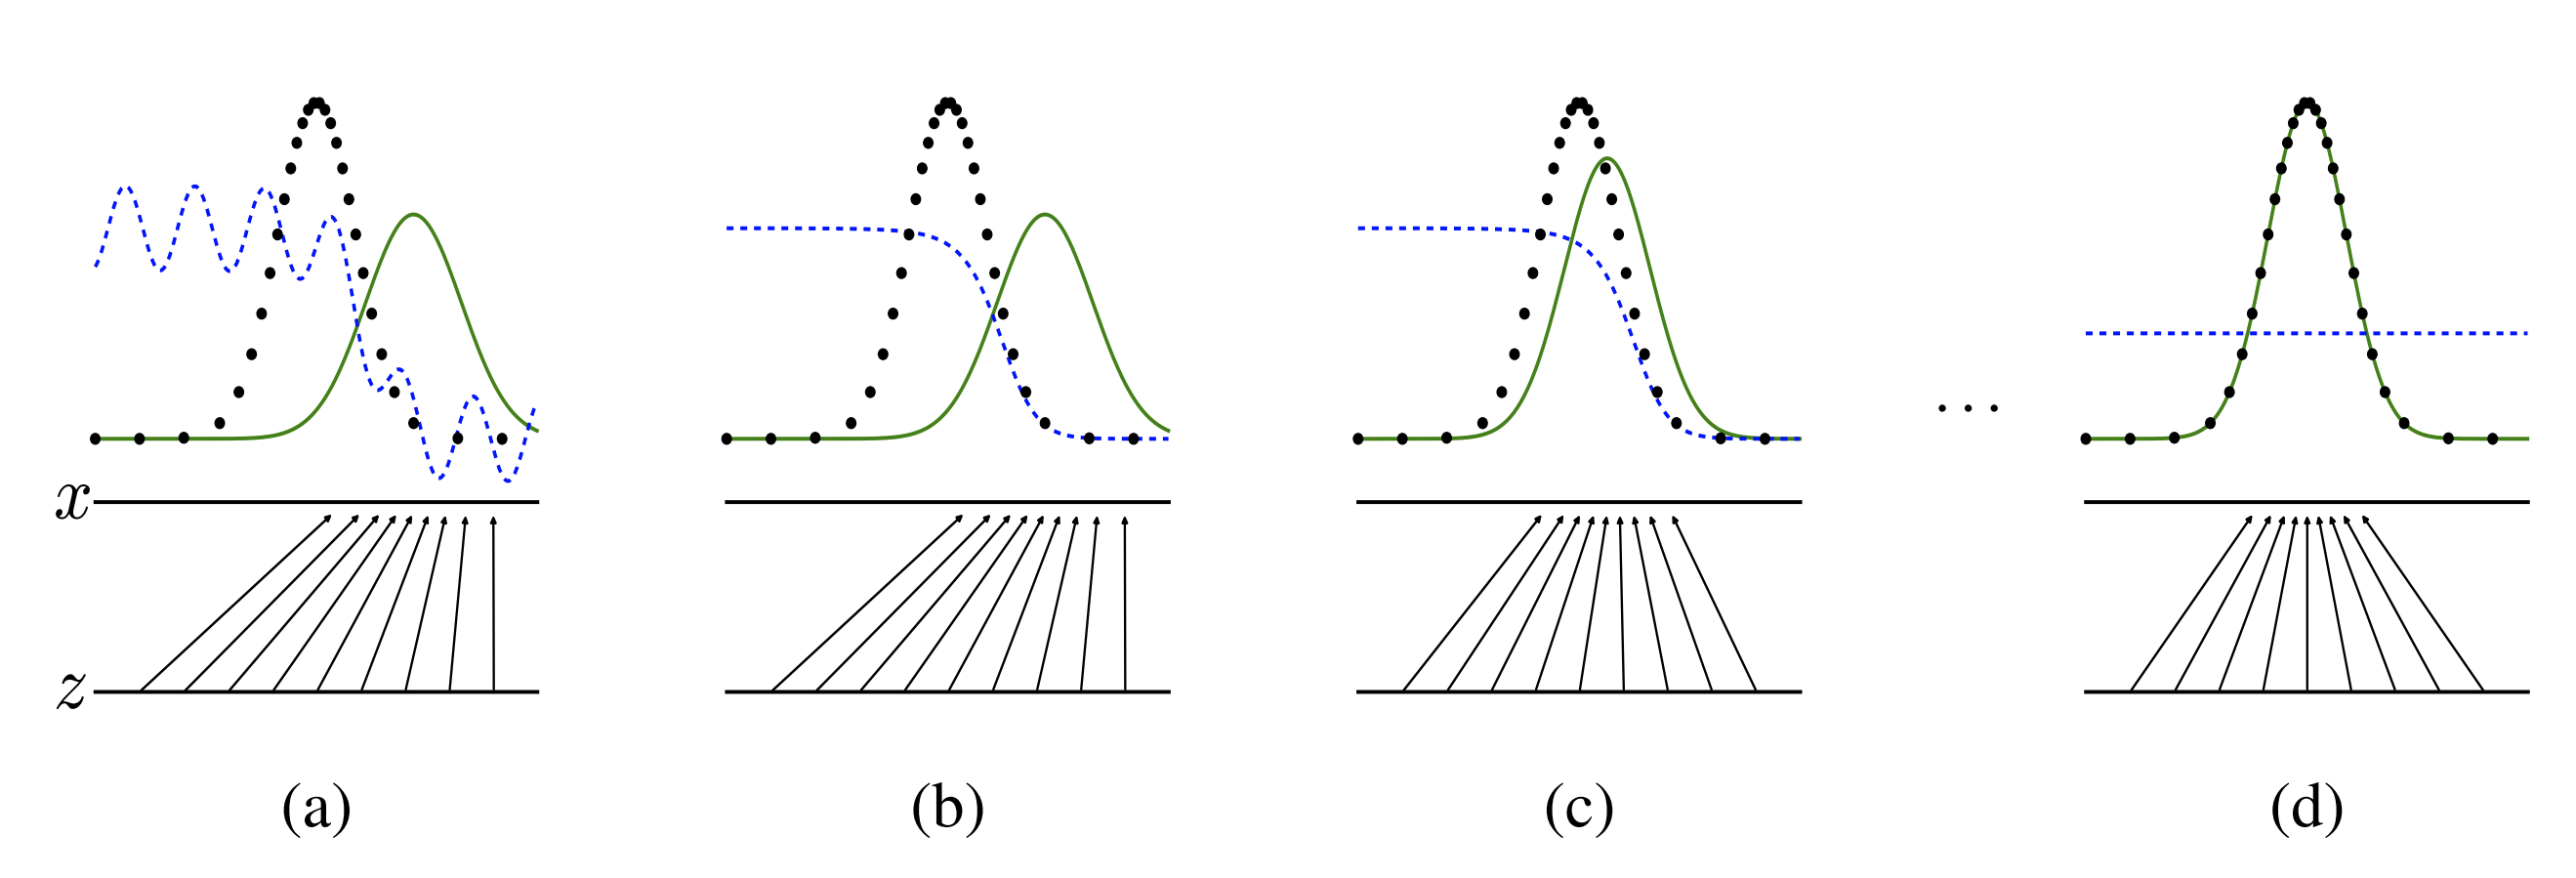
\includegraphics{plots/trainingGAN.png}}
\tiny{\\GANs are trained by simultaneously updating the discriminative distribution
(D, blue, dashed line) so that it discriminates between samples from the data generating distribution (black,dotted line) $p_x$ from those of the generative distribution $p_g (G)$ (green, solid line).Source: Goodfellow et al (2017)}
\end{figure}
\begin{itemize}
\item For $k$ steps, G's parameters are frozen and one performs \textbf{gradient ascent} on D to increase its accuracy.
\item Finally, D's parameters are frozen and one performs \textbf{gradient descent} on G to increase its generation performance. %/ to make D misclassify.
\item Note, that G gets to peek at D's internals (from the back-propagated errors) but D  does not get to peek at G.
\end{itemize}
\end{frame}

\begin{frame} {Divergence measures}
  \begin{itemize}
    \item The goal of generative modeling is to learn $p_{\text{data}}(\mathbf{x})$.
    \vspace{2mm}
    \item The differences between different generative models can be measured in terms of \textbf{divergence measures}.
    \vspace{2mm}
    \item A divergence measure quantifies the distance between two distributions. %It is a measure of how different one distribution is from another.
    \vspace{2mm}
    \item There are many different divergence measures that one can us (e.g. Kullback-Leibler divergence).
    \vspace{2mm}
    \item All such measures always  positive and  0 if and only if the two distributions are equal to each other.
  \end{itemize}
\end{frame}

\begin{frame} {Divergence measures}
  \begin{itemize}
    \small{\item One approach to training generative models is to explicitly minimize the distance between $p_{\text{data}}(\xv)$ and the model distribution $p_{\theta}(\xv)$ according to some divergence measure.
    \vspace{2mm}
    \item If our generator has the capacity to model $p_{\text{data}}(\xv)$ perfectly, the choice of divergence does not matter much because they all achieve their minimum (that is 0) when $p_{\theta}(\xv) = p_{\text{data}}(\xv)$.
    \vspace{2mm}
    \item However, it is not likely that that the generator, which is  parametrized by the weights of a neural network, is capable of perfectly modelling an arbitrary $ p_{\text{data}}(\xv)$.
    \vspace{2mm}
    \item In such a scenario, the choice of divergence measure matters, because the parameters that miniminize the various divergence measures differ.}
  \end{itemize}
\end{frame}

\begin{frame} {Implicit Divergence measure of GANs}
  \begin{itemize}
   \item GANs do not explicitly minimize any divergence measure.
   \item However, (under some assumptions!) optimizing the minimax loss is equivalent to implicitly minimizing a divergence measure.
    \item That is, if the optimal discriminator is found in every iteration,  the generator minimizes %a divergence measure between distributions known as
    the  \textbf{Jensen-Shannon divergence  (JSD)} (theorem and proof are given by the original GAN paper (Goodfellow et al, 2014)):
    \begin{align*}
      JS(p_{\text{data}}||p_g) & =  \frac{1}{2} KL(p_{\text{data}}||\frac{p_{\text{data}}+p_g}{2}) + \frac{1}{2}  KL(p_g || \frac {p_{\text{data}} + p_g}{2}) \\
        KL(p_{\text{data}}||p_g) & = E_{\xv \sim p_{\text{data}}(\xv)}[log \frac {p_{\text{data}}(\xv)}{p_g(\xv)}]
    \end{align*}
 % \vspace{2mm}
%    \item A generator with sufficient capacity successfully learns the target distribution
 % \vspace{2mm}
 %   \item Otherwise, it exhibits "mode-seeking" behaviour.
%  \vspace{2mm}
%    \item Researchers originally speculated that this behaviour is the reason GANs produce stunningly realistic samples.
  \end{itemize}
\end{frame}


\begin{frame} {Optimal Discriminator}

  For G fixed, the optimal discriminator $D^*_G$ is:
  \begin{figure}
    \centering
      \scalebox{1}{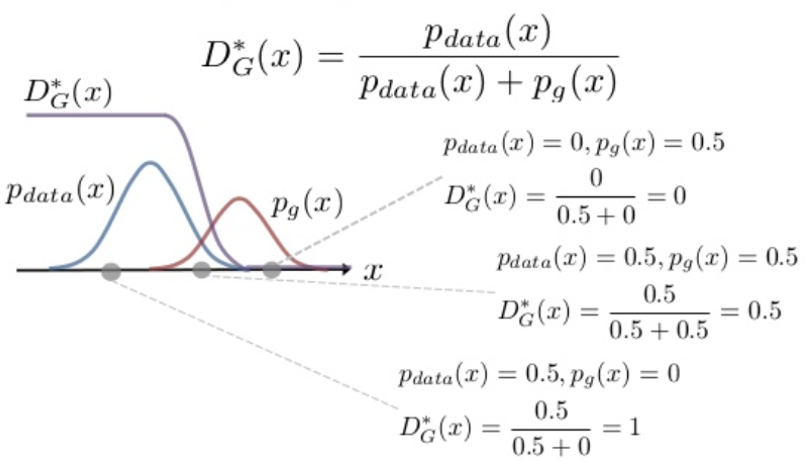
\includegraphics[width=7cm]{plots/opt_discriminator.png}}
      \tiny{\\Credit: Mark Chang}
  \end{figure}
   \begin{itemize}
  \item  The optimal discriminator returns a value greater than 0.5 if the probability to come from the data ($p_{data}(x)$)  is larger than the probability to come from the generator ($p_g(x)$).
  \end{itemize}
\end{frame}

\begin{frame} {Optimal Discriminator}

  For G fixed, the optimal discriminator $D^*_G$ is:
  \begin{figure}
    \centering
      \scalebox{1}{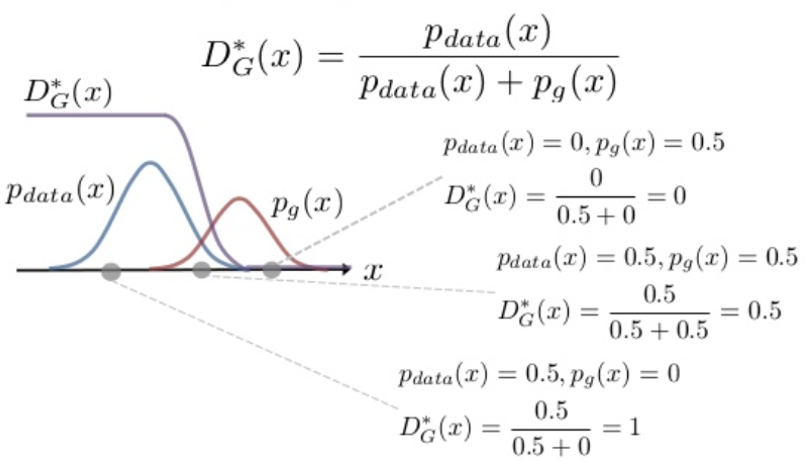
\includegraphics[width=7cm]{plots/opt_discriminator.png}}
      \tiny{\\Credit: Mark Chang}
  \end{figure}
  \begin{itemize}
  \item  Note: The optimal solution is almost never found in practice, since the discriminator has a finite capacity and is trained on a finite amount of data.
  \item Therefore, the assumption needed to guarantee that the generator minimizes the JSD does usually not hold in practice.
  \end{itemize}
\end{frame}

%

%--------------------------------------------
%
%---------------------------------------------


\begin{vbframe}
\frametitle{References}
\footnotesize{
\begin{thebibliography}{99}
\bibitem[Goodfellow et al., 2014]{5} Ian J. Goodfellow, Jean Pouget-Abadie, Mehdi Mirza, Bing Xu, David Warde-Farley, Sherjil Ozair, Aaron Courville, Yoshua Bengio (2014)
\newblock Generative Adversarial Networks
\newblock \emph{\url{https://arxiv.org/abs/1406.2661}}
%%%%%%%%%%%%%%%%%%%%%%%%%%%%%%%%%%
%%%%%%%%%%%%%%%%%%%%%%%%%%%%%%%%%
\bibitem[Goodfellow, 2016]{7} Ian Goodfellow (2016)
\newblock NIPS 2016 Tutorial: Generative Adversarial Networks
\newblock \emph{\url{https://arxiv.org/abs/1701.00160}}
%%%%%%%%%%%%%%%%%%%%%%%%%%%%%%%%%%
%%%%%%%%%%%%%%%%%%%%%%%%%%%%%%%%%
\bibitem[Chang, 2016]{9} Mark Chang (2016)
\newblock Generative Adversarial Networks
\newblock \emph{\url{https://www.slideshare.net/ckmarkohchang/generative-adversarial-networks}}
%%%%%%%%%%%%%%%%%%%%%%%%%%%%%%%%%%
%%%%%%%%%%%%%%%%%%%%%%%%%%%%%%%%%

%%%%%%%%%%%%%%%%%%%%%%%%%%%%%%%%%%%%%%%%%%%%%%%%%%%%%%%%%%%%%%%%%%
%%%%%%%%%%%%%%%%%%%%%%%%%%%%%%%%%%%%%%%%%%%%%%%%%%%%%%%%%%%%%%%%%%

\end{thebibliography}
}
\end{vbframe}

\endlecture
\end{document}
